\documentclass[a4paper, 11pt]{article}
\usepackage{fullpage, amssymb, amsmath, graphicx, hyperref} 

\newcommand{\mytitle}{Problem Set 1}

\begin{document}
\noindent
\large\textbf{\mytitle} \\ \\ Tyler Gordon \\
\normalsize \today 
\ \ \hrulefill
\section*{Problem 1}
	\subsection*{Part A}
		\href{http://www.github.com/tagordon/ASTR-507}{On github: http://github.com/tagordon/ASTR-507}
	\subsection*{Part B}
		Initial configuration: 
		\ \\ \\
		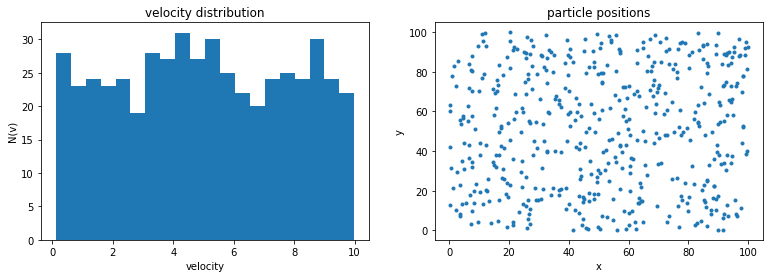
\includegraphics[width=15cm]{before.png}
		\ \\ \\
		Final configuration:
		\ \\ \\
		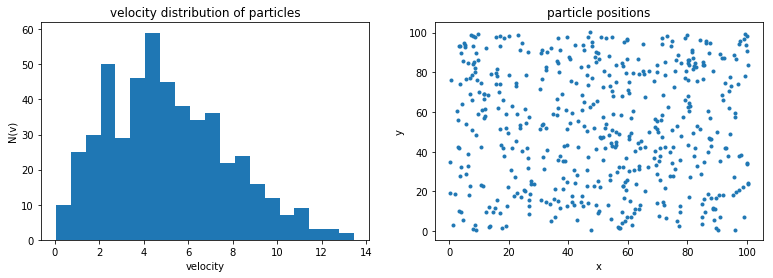
\includegraphics[width=15cm]{after.png}
		\pagebreak
\section*{Problem 2}
	\subsection*{Part A}
		\textbf{Deriving the Maxwellian velocity distribution:}
		\ \\ \\
		$dN = f(p)dp_xdp_y$ gives the number of particles with momentum between $p_x$ and $p_x + dp_x$, and 
		$p_y$ and $p_y + dp_y$. 
		Starting with this expression, 
		we have:
		\begin{equation*}
			dN = f(p)dp \propto e^{-E/kT}dp_xdp_y = e^{-m(v_x^2+v_y^2)/2kT}m^2dv_xdv_y
		\end{equation*}
		rewriting this in polar coordinates, we get
		\begin{equation*}
			dN \propto e^{-mv^2/2kT}m^2vdvd\theta
		\end{equation*}
		Integrating over all directions introduces a factor of $2\pi$:
		\begin{equation*}
			dN \propto 2\pi e^{-mv^2/kT}m^2vdv
		\end{equation*}
		We now must normalize such that the total number of particles is 1. By integrating $dN$ over all velocities from 
		zero to infinity, we find that the normalization constant must be $2m/kT$ from which we find the final distribution:
		\begin{equation*}
			\frac{dN}{dv} = \frac{2m}{kT}ve^{-mv^2/kT}
		\end{equation*}
		\ \\ \\
		\textbf{Deriving the Maxwellian energy distribution:}
		\ \\ \\
		The number of particles with energy between $E$ and $E + dE$ is given by $dN = f(p)dE$:
		\begin{equation*}
			dN \propto e^{-E/kT}dE
		\end{equation*}
		Normalizing this, we find:
		\begin{equation*}
			\frac{dN}{dE} = \frac{e^{-E/kT}}{kT}
		\end{equation*}
	\subsection*{Part B}
		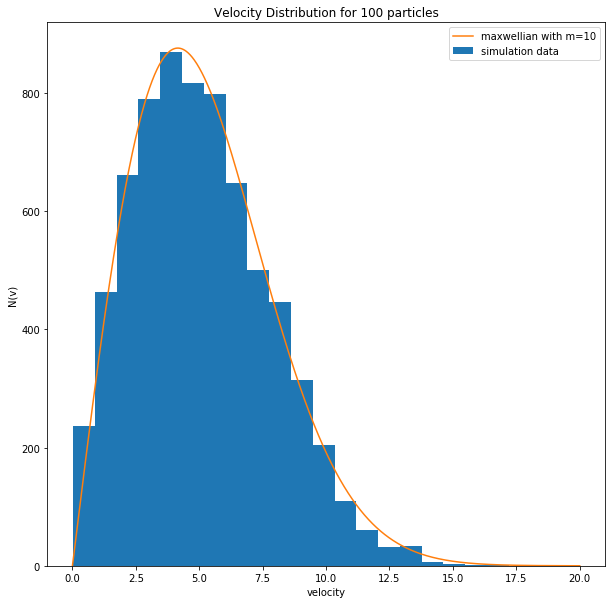
\includegraphics[width=15cm]{maxwellian.png}
	\subsection*{Part C}
		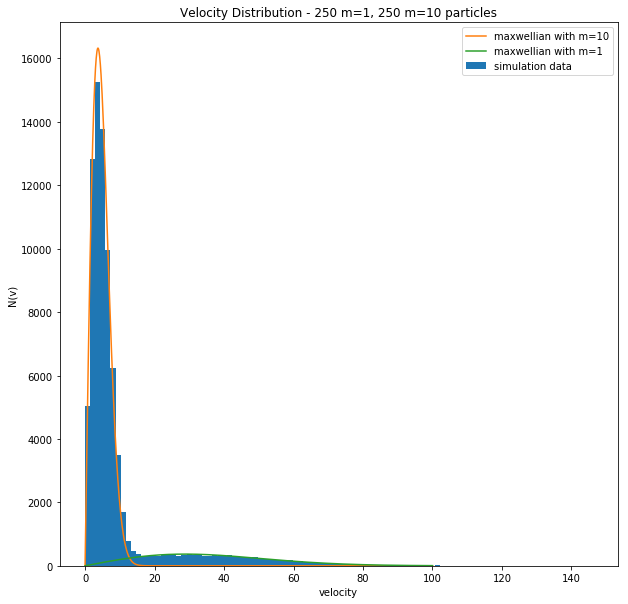
\includegraphics[width=15cm]{two_maxwellian.png}
		\ \\ \\
		Each type of particle ($m=1$ vs. $m=10$) has a separate Maxwellian velocity distribution. This is the expected 
		behavior - the more massive particles come from the same Maxwellian distribution in energy as do the less massive 
		particles, but because of their mass, they have smaller velocities for the same energies. Thus in velocity, the two 
		populations each have their own Maxwellian distribution. 
\section*{Problem 3}
	\subsection*{Part A}
		A \emph{very} rough criterion could be arrived at by computing the difference between the population in two 
		widely different energy bins and checking that it is approximately the difference expected from the Maxwellian 
		distribution, to within some specified error. i.e. how long does it take for the energies to be distributed approximately 
		according to the Maxwellian distribution? To make this criterion more robust to the small number of particles in my 
		simulations, I can split the velocities in half at some cutoff, and consider the number of particles with velocities 
		greater than $v_\text{cut}$ versus the number of particles with velocities less than $v_\text{cut}$. 
	\subsection*{Part B}
		Since the particles need to collide to "communicate" their velocities to each other, the time to relax should scale with 
		the time between collisions. The mean free path in three dimensions is given by $l=1/\sigma n$ where $\sigma$ is 
		the cross section of the 
		particles and $n$ is the number density of particles. The time between collisions for a particle with velocity v is thus $
		\tau = 1/\sigma n v$. In two dimensions, the cross section is actually the linear extent of the particle, or twice its radius. 
	\subsection*{Part C}
		If we choose to split the 2-D Maxwellian at $v = \sqrt{2\ln2}v_\text{max}$ where $v_\text{max}$ is the maximum of 
		the velocity distribution at $v_\text{max} = \sqrt{m/2kT}$ 
		then we get the same population on each side of the velocity cut. We can use this expectation to test for the system 
		being relaxed. I'll arbitrarily consider the system to be relaxed when the populations on either side of this cut are within 
		ten percent of each other. 
		\ \\ \\
		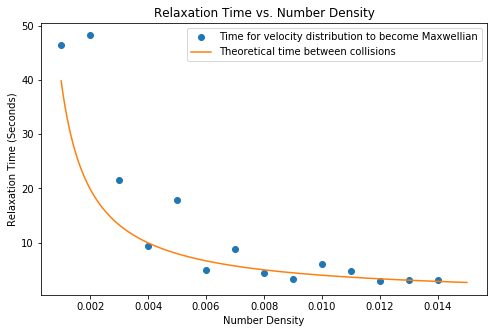
\includegraphics[width=15cm]{relaxation_v_density.png}
		\ \\ \\
		This plot demonstrates that my numerical criterion for relaxation scales with number density 
		the same as my theoretical criterion: the average time between collisions. In fact, the two criteria correspond 
		rather closely, 
		showing that they not only scale the same, but that the velocity distribution approaches a Maxwellian on the same 
		timescale as the average time between collisions for the system. 
		\ \\ \\
		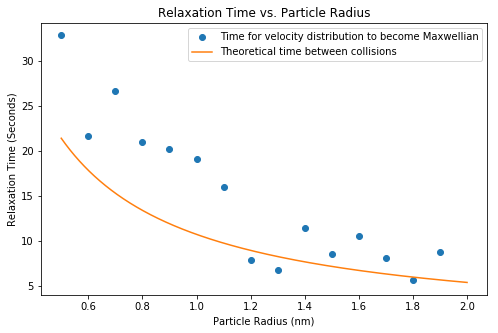
\includegraphics[width=15cm]{relaxation_v_radius.png}
		\ \\ \\
		This plot demonstrates that my numerical relaxation criterion scales with particle radius in the same way as my 
		theoretical criterion. The correlation between the two is not as clear as in the relaxation vs. number density plot, 
		but the timescales appear to be similar. 
	\subsection*{Part D}
		The first plot shows the linear relationship between pressure and temperature which we expect from the ideal 
		gas law. The second shows the linear relationship between pressure and number density. 
		\ \\ \\
		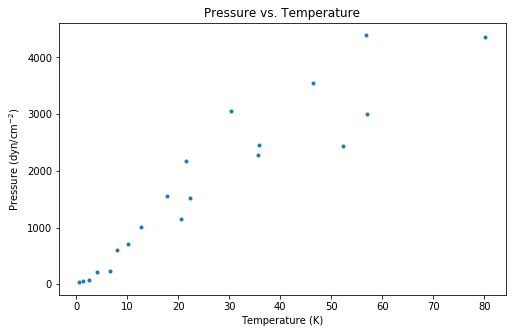
\includegraphics[width=15cm]{pressure_v_temp.png}
		\ \\ \\
		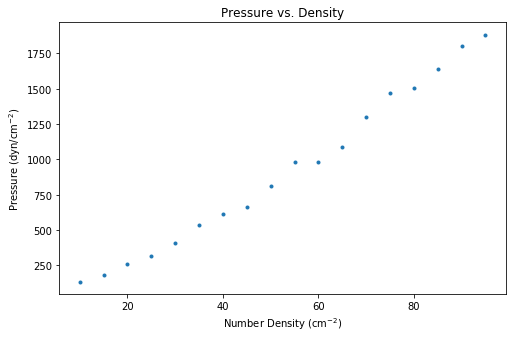
\includegraphics[width=15cm]{pressure_v_dens.png}
		\ \\ \\
		The temperature plot shows a large scatter at higher temperatures. I think that this is because I computed 
		temperature from the maximum of the velocity distribution using $v_\text{max} = \sqrt{2kT/m}$. For more energetic 
		simulations, there is a large scatter in velocities, and the corresponding computed temperature is also more 
		uncertain. 
\end{document}
